\newpage % Rozdziały zaczynamy od nowej strony.
\section{Generowanie podpisów do obrazów -- aktualne rozwiązania}
W celu wygenerowania podpisu do obrazu przy użyciu algorytmów uczenia maszynowego wykorzystuje się sieci neuronowe. Sam proces generowania podpisów można rozbić na dwa etapy: przetwarzanie obrazu oraz generowanie tekstu. Z tego względu najpopularniejsze podejścia wykorzystują połączenia sieci wykorzystywanych do przetwarzania obrazów wraz z sieciami wykorzystywanymi do przetwarzania języka naturalnego. Takie podejście wyodrębnia dwa główne moduły w całej architekturze sieci:
\begin{itemize}
  \item moduł kodujący obraz -- jego danymi wejściowymi jest obraz w postaci macierzy pikseli, natomiast wyjściem jest wektor sprowadzony do postaci zgodnej z formatem wejściowym modułu dekodującego,
  \item moduł dekodujący zakodowany wcześniej obraz -- wejściem tego modułu jest wyjście modułu kodującego, natomiast wyjściem jest ostatecznie wygenerowane zdanie.
\end{itemize}
\begin{figure}[H]
  \centering
  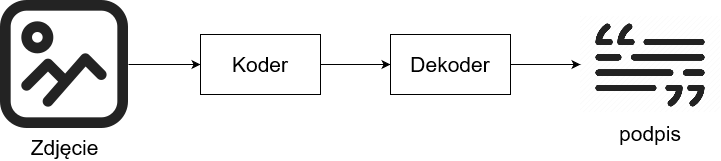
\includegraphics[width=.9\linewidth]{diagram}
  \caption{Typowa architektura generatora podpisów. Opracowanie własne}
  \label{fig:schemat-captioning}
\end{figure}
\subsection{Moduły kodujące}
Ze względu na niezwykle dużą skuteczność, jak również popularność, najczęściej wykorzystywaną siecią neuronową jako moduł kodujący jest splotowa sieć neuronowa. Główną jej modyfikacją, w celu dostosowania do problemu, jakim jest generowanie podpisów, jest dopasowanie ostatnich warstw w taki sposób, aby~ostateczny wektor wyjściowy był kompatybilny z typowym formatem danych wejściowych sieci wykorzystywanych w dziedzinie przetwarzania języka naturalnego.
\subsubsection{Bardzo głębokie sieci splotowe}
Jednym z częściej wykorzystywanych rodzajów sieci splotowej są głębokie sieci neuronowe. Charakteryzują się one dużą liczbą warstw splotowych oraz małymi wielkościami filtrów. Aktualnie istnieje wiele architektur wykorzystujących takie podejście. Jedną z pierwszych była sieć VGGNet \cite{vggnet}. Dzięki zastosowaniu dużej liczby warstw splotowych możliwe było klasyfikowanie obrazów o dużej rozdzielczości z bardzo wysoką skutecznością. Dużym minusem tego rodzaju sieci są wymagane zasoby. Ze względu na dużą ilość warstw konieczna jest alokacja dużej ilości pamięci w jednostce GPU, a samo przetworzenie danych przez sieć wymaga wielu obliczeń.
\subsubsection{Transformer wizyjny}
Transformer wizyjny \cite{vit} to model przetwarzania obrazów, który różni się od tradycyjnych architektur zawierających sieci splotowe. Opiera się on na transformerze znanym głównie z zastosowań w przetwarzaniu języka naturalnego. Przy jego pomocy obraz jest przetwarzany poprzez podzielenie na nienachodzące się bloki, a każdy blok reprezentowany jest jako token, podobnie jak słowa w zdaniu. Te tokeny są traktowane jako sekwencja wejściowa dla modelu transformera. Poglądowy diagram przedstawiający architekturę transformera wizyjnego został przedstawiony na rysunku \ref{fig:vit-architecture}.
\begin{figure}[H]
  \centering
  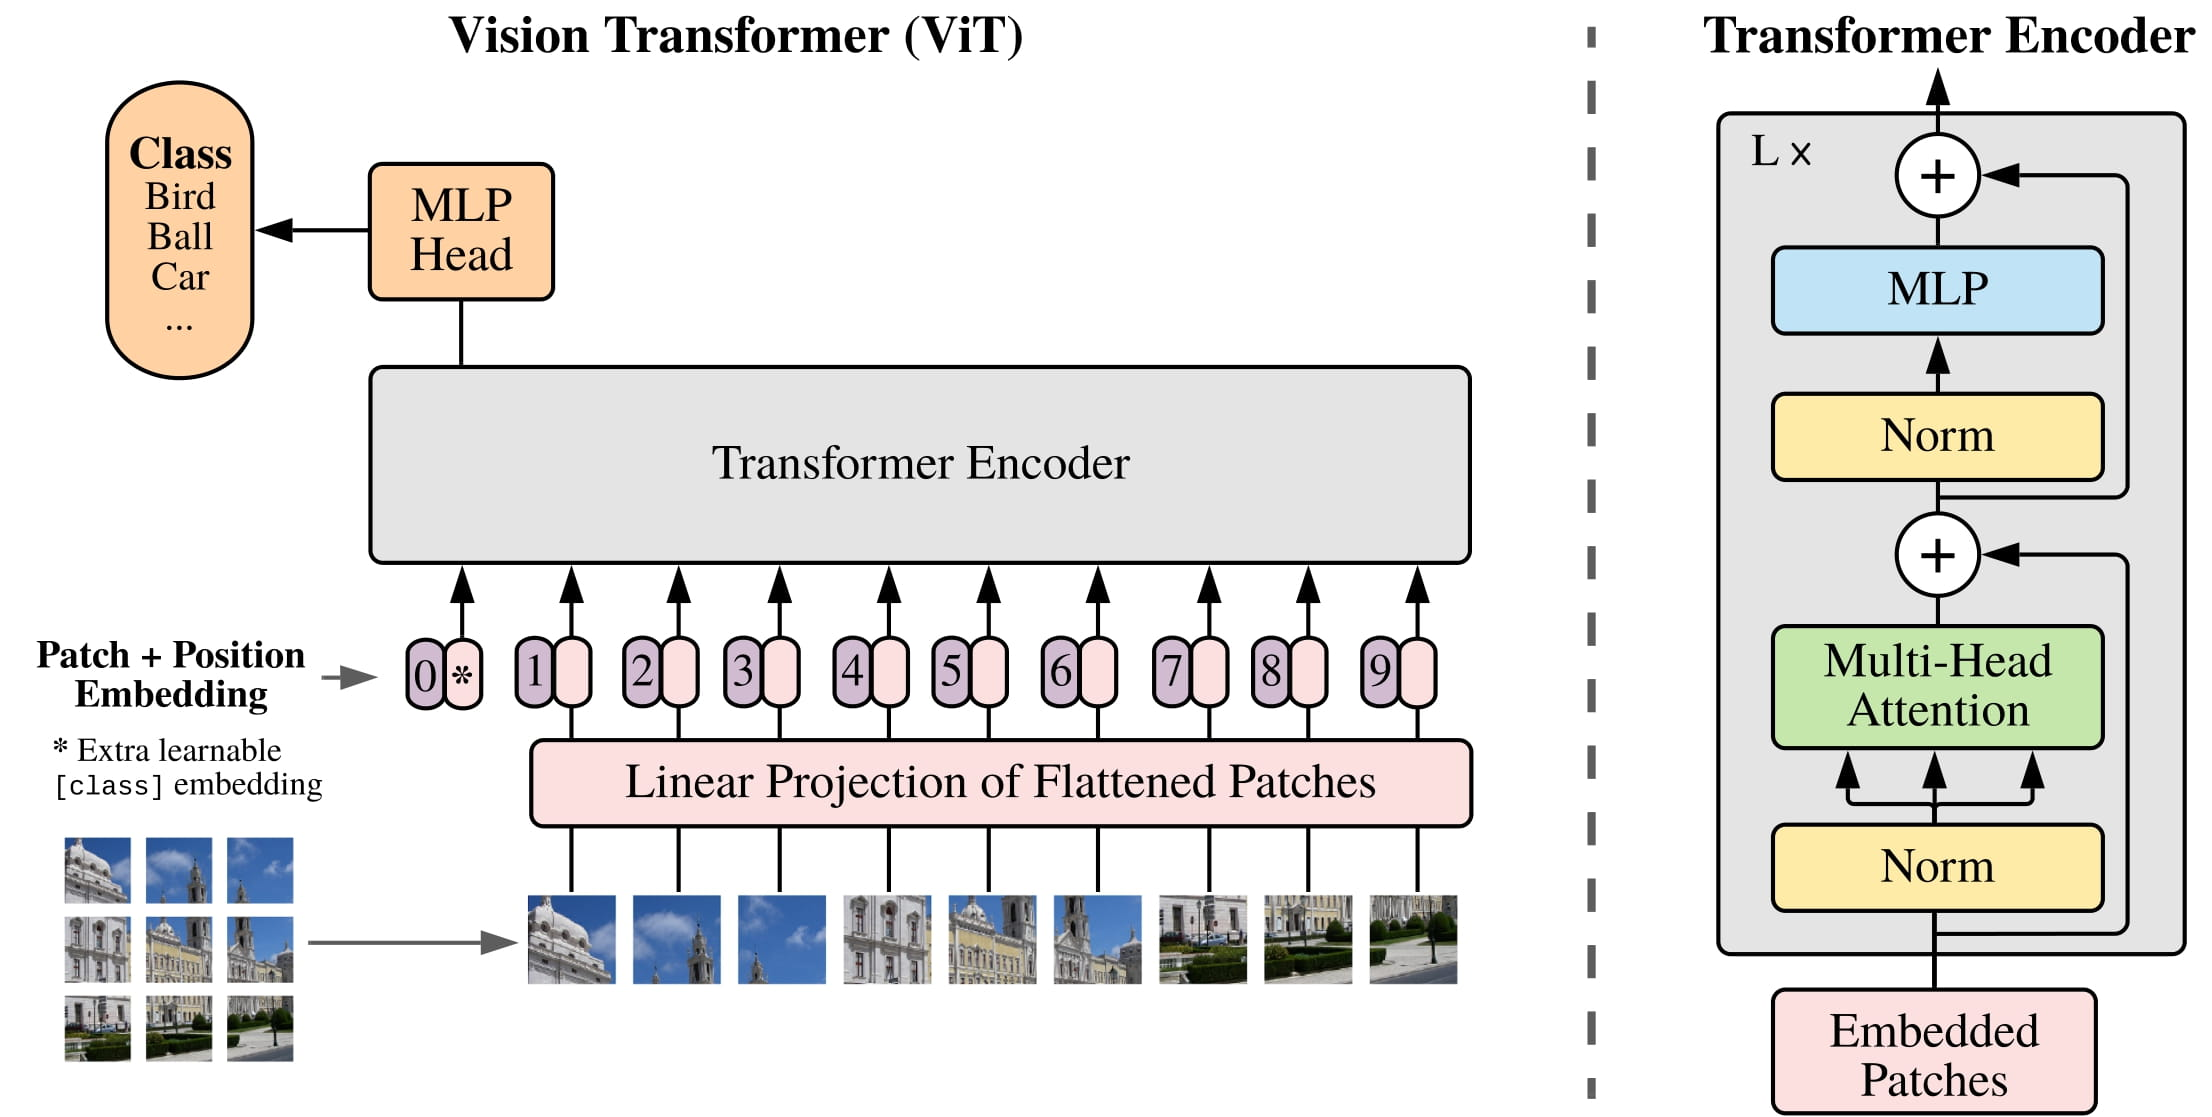
\includegraphics[width=.95\linewidth]{vit_architecture}
  \caption{Diagram architektury transformera wizyjnego. Źródło: \cite{vit}}
  \label{fig:vit-architecture}
\end{figure}
\noindent Dane wyjściowe z kodera transformera przetwarzane są w bardzo podobny sposób jak w przypadku danych wyjściowych głębokich warstw sieci splotowych -- przy pomocy w pełni połączonych warstw, wektor wyjściowy jest sprowadzany do postaci wektora zawierającego odpowiednie klasy, co zostało przedstawione na diagramie przy pomocy bloku ,,MLP Head'' oraz ,,Class''. W dziedzinie generowania podpisów do obrazków wspomniane bloki najczęściej zostają pominięte, dzięki czemu danymi wyjściowymi jest wektor zawierający informacje o obrazie, który jest wykorzystywany jako wejście dla modułu dekodującego.
\subsection{Moduły dekodujące}
Dzięki sprowadzeniu obrazu do formatu zwykłego wektora poprzez moduł kodujący możliwe jest wykorzystanie większości rozwiązań dedykowanych do zwykłych zadań przetwarzania języka naturalnego. Jako analogiczną dziedzinę można tutaj wyróżnić zagadnienie związane z generowaniem odpowiedzi na pytania -- główną różnicą w przypadku generowania podpisów jest sprowadzenie obrazu do wartości możliwej do przetworzenia przez moduł kodujący. W przypadku zagadnień związanych z generowaniem odpowiedzi, przetwarzany jest tekst, natomiast w przypadku generowania podpisów są to obrazu. Dalsza część architektury, czyli moduł kodujący, jest analogiczna w obu przypadkach. Częstym wyborem jako moduł dekodujący jest podstawowa rekurencyjna sieć neuronowa -- RNN \cite{rnn}. W przypadku takiej sieci wektor będący wyjściem modułu kodującego służy jako pierwszy element wejściowy modułu dekodującego. Naturalnie możliwe jest wykorzystywanie bardziej zaawansowanych odmian sieci rekurencyjnej jak LSTM \cite{lstm} oraz GRU \cite{gru}. Również wykorzystywane są moduły atencji \cite{attention} \cite{attentionImageCaptioning}, w których przypadku szczególnie użyteczne są głębokie sieci neuronowe. Wyniki z poprzednich warstw splotowych służą jako kontekst, z którego może korzystać moduł atencji.
\subsubsection{Transformer}
% MAYBE rozwinąć
Tak jak w przypadku pozostałych problemów związanych z przetwarzaniem języka naturalnego, również w kontekście generowania podpisów do obrazów, popularnością cieszy się sieć Transformer \cite{transformer}. Główną różnicą w porównaniu do klasycznych sieci rekurencyjnych jest przetwarzanie przez transformer sekwencji w całości, a nie pojedynczych jej elementów. Takie działanie jest możliwe dzięki zastosowaniu modułu atencji oraz zakodowania pozycyjnego, czyli dodania informacji o pozycji elementu w sekwencji do jego wartości. Sama atencja pozwala na określenie znaczenia danych elementów sekwencji w kontekście jej całości. Jest to znacząca przewaga nad sieciami rekurencyjnymi, które biorą pod uwagę jedynie aktualnie przetwarzany element oraz dane wygenerowane na podstawie wszystkich wcześniej przetworzonych elementów. Wykorzystanie tych rozwiązań również niweluje całkowicie problem eksplozji lub zanikania gradientu, który występuje w przypadku sieci rekurencyjnych.

\subsection{Neuronowy generator podpisów obrazów -- NIC}
Architektura NIC \cite{nic} (ang. Neural Image Caption) wykorzystuje połączenie splotowej sieci neuronowej \cite{ioffe2015batch} oraz sieć LSTM, w celu generowania podpisów. Osiąga ona wartość BLEU-4 na poziomie 0,27 dla zbioru MS COCO \cite{mscoco}. Jest to stosunkowo stare rozwiązanie pochodzące z 2015 roku, ale mimo to skuteczność tejże architektury nie odbiega znacząco od wyników aktualnych rozwiązań. Samo połączenie splotowej sieci neuronowej wraz z siecią rekurencyjną w architekturze NIC zostało zaimplementowane w nieskomplikowany sposób: pierwszym elementem wejściowym sieci LSTM jest zakodowany obraz otrzymany poprzez przetworzenie go przez sieć splotową. Autorzy pracy zastosowali technikę transferu wiedzy i ograniczyli trenowanie sieci jedynie do modułu dekodującego -- obrazy zostały zakodowane tylko raz, po czym posłużyły za dane treningowe dla sieci LSTM. Przy takim podejściu kluczowy był odpowiedni wybór modułu kodującego, dlatego autorzy zdecydowali się na wybór modelu osiągającego wysokie wyniki w wielu różnych dziedzinach przetwarzania obrazów. Taki model można uznać za wysoce generalizujący, a co za tym idzie, posiadający lepsze predyspozycje adaptacji do innych zadań, co jest idealnym przypadkiem wykorzystania jako moduł w sieci generowania podpisów, czyli zadania odbiegającego znacząco od klasycznych zastosowań sieci splotowych.

\subsection{Generatywny transformator obrazu na tekst -- GIT}
Bardziej rozbudowana architektura GIT \cite{wang2022git} (ang. Generative Image-to-text Transformer), w porównaniu do architektury NIC, na zbiorze danych MS COCO osiągnęła wartość metryki BLEU-4 równą 0,43 -- wynik o 50\% lepszy. Wykorzystuje ona model Transformera wizyjnego jako moduł kodujący wraz z klasycznym Transformerem wykorzystanym jako moduł dekodujący. Rozwiązanie to pochodzi z 2022 roku i aktualnie osiąga jedne z najlepszych wyników w dziedzinie generowania podpisów do obrazków. Autorzy główną uwagę skupili na skonstruowaniu prostej architektury wykorzystującej tylko jeden moduł kodujący i dekodujący -- wiele architektur w odróżnieniu od modelu GIT wykorzystuje kilka modułów pracujących równolegle. Tak dobre wyniki mimo dużej prostoty architektury zostały osiągnięte między innymi poprzez zastosowanie wcześniej wytrenowanego modelu Transformera wizyjnego na ogromnym zbiorze danych.
% TODO rozwinąć

\subsection{Raz na zawsze -- OFA}
Architektura OFA \cite{wang2022ofa} (ang. Once for all) została stworzona z myślą o wielozadaniowości, dzięki czemu jest w stanie rozwiązać wiele zadań związanych z przetwarzaniem obrazów cyfrowych, w tym generowania podpisów. Model ten nie jest ograniczony jedynie do przetwarzania obrazów, ponieważ opiera się on na metodzie seq2seq, polegającej na przetwarzaniu pewnej sekwencji do innej sekwencji. Jego danymi wejściowymi są dane językowe, którym może towarzyszyć obraz, z tego względu oprócz macierzy pikseli danego obrazka konieczne jest również podanie tekstu w postaci formuły informującej architekturę o konieczności wygenerowania podpisu jak na przykład „co opisuje obraz?”. Wszelkie typy zadań rozwiązywane przez architekturę OFA zostały zobrazowane na rysunku \ref{fig:ofa-tasks} stworzonym przez autorów sieci.
\begin{figure}[H]
  \centering
  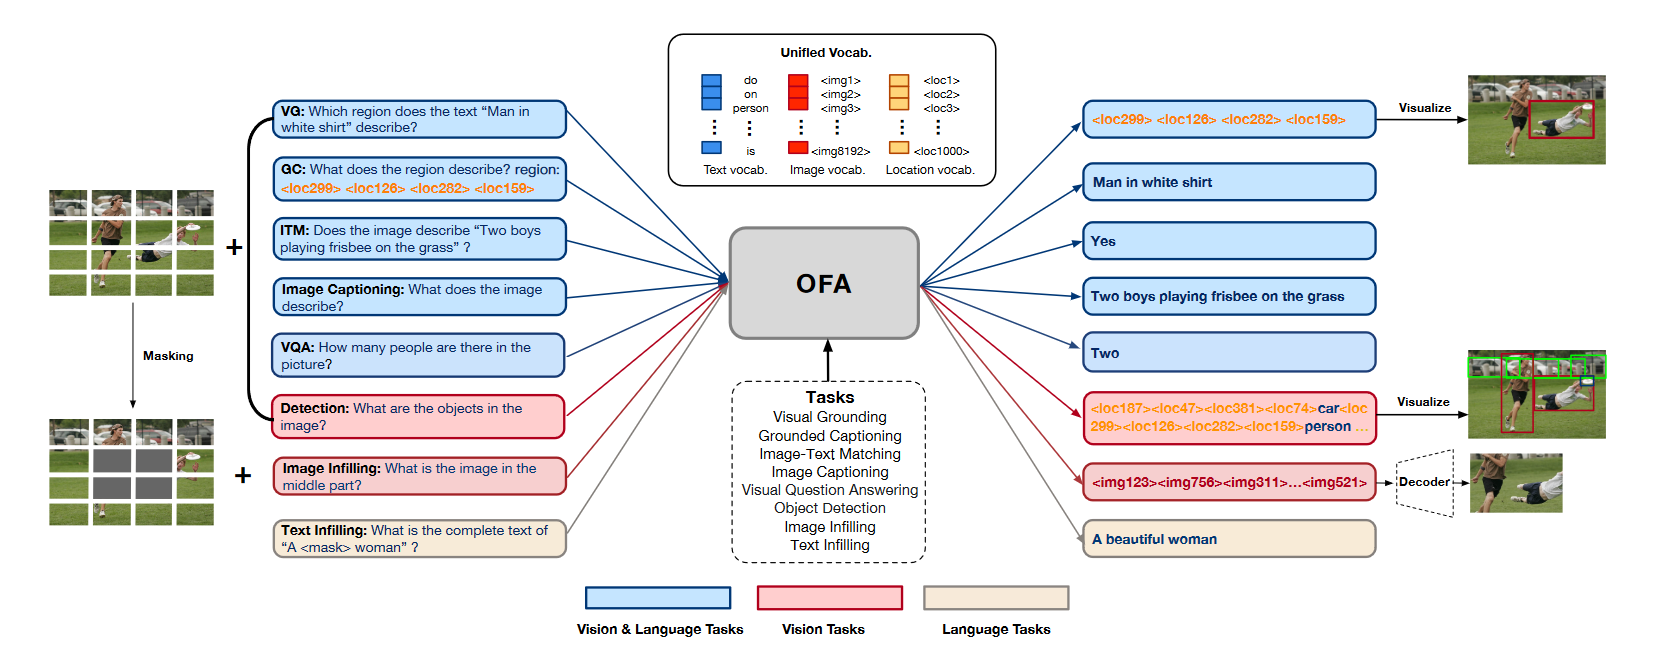
\includegraphics[width=\linewidth]{ofa_tasks}
  \caption{Diagram przedstawiający możliwe typy zadań rozwiązywane przez architekturę OFA. Źródło: \cite{wang2022ofa}}
  \label{fig:ofa-tasks}
\end{figure}
\noindent Architektura osiągnęła skuteczność na poziomie 0,44 dla metryki BLEU-4 na zbiorze danych MS COCO, co jest wynikiem porównywalnym do architektury GIT. Niemniej jednak wynik ten jest bardziej imponujący niż w przypadku modelu GIT, ponieważ architektura OFA jest w stanie rozwiązać wiele zadań związanych nie tylko z przetwarzaniem obrazów bez konieczności ponownego dostrajania modelu.

\subsection{Ujednolicone wstępne uczenie modeli generowania podpisów -- VLP}
Architektura VLP \cite{vlp} (ang. Vision-language Pre-training model) różni się tym od pozostałych rozwiązań, iż nie składa się z oddzielonych od siebie modułu kodującego oraz dekodującego -- przetwarzanie obrazu oraz generowanie tekstu odbywa się w ramach tej samej jednostki wykorzystującej zmodyfikowaną architekturę transformera. Dodatkowo architektura została stworzona z myślą o wykorzystywaniu jej do różnego rodzaju zadań. Sami autorzy wyodrębnili dwa: generowanie podpisów oraz odpowiadanie na pytania w odniesieniu do obrazu. Z tego względu samo uczenie architektury przebiegało w trzech etapach:
\begin{itemize}
  \item przetworzenie obrazu przy pomocy sieci splotowej rozpoznającej obiekty znajdujące się na obrazie.
  \item Zakodowanie zdania wraz z obrazem w postaci wektora, który posłużył jako wartość wejściowa dla architektury transformera.
  \item Dostrojenie architektury transformera w celu dostosowania jej do konkretnego zadania.
\end{itemize}
Mimo iż autorzy zastosowali technikę przetwarzania jednocześnie zdania oraz obrazu, konieczne było w pierwszej kolejności zakodowanie danych wizualnych, co zostało wykonane przy pomocy sieci splotowej. Architektura osiągnęła skuteczność na poziomie 0,39 dla metryki BLEU-4 na zbiorze MS COCO. Jest to wynik niższy niż osiągnięty przez architektury GIT oraz OFA, jednakże różnica nie jest drastyczna.

\subsection{Szybkie generowanie podpisów obrazów z wyrównaniem pozycji -- FNIC}
Architektura FNIC \cite{fnic} (ang. Fast Neural Image Caption) wyróżnia się na tle pozostałych rozwiązań niewykorzystaniem klasycznego podejścia w przetwarzaniu języka naturalnego, które oparte jest na sieci rekurencyjnej, czyli przetwarzaniu kolejnych elementów sekwencji. Takie podejście jest niezwykle skuteczne, ponieważ pozwala na generowanie kolejnych elementów z uwzględnieniem informacji o pozostałych już wygenerowanych pozycjach, czy też całej sekwencji w przypadku wykorzystywania modułu atencji. Jednakże wiążę się to z pojedynczym przetwarzaniem każdego z elementów, a co za tym idzie, znacząco wpływa na czas potrzebny do takiego przetworzenia. Architektura FNIC, w celu przyspieszenia generowania podpisów, wykorzystuje technikę zwaną wyrównaniem pozycji. W pierwszej kolejności obraz przetwarzany jest przy pomocy sieci splotowej do postaci wektora, co jest najpopularniejszą metodą przetworzenia obrazu do postaci wejściowej do dalszej analizy. Następnie informacje o obrazie są przetwarzane przez sieć rekurencyjną GRU, w celu wygenerowania pojedynczych słów, które mogą opisywać obraz -- głównym celem tego modułu jest to, aby wygenerowane słowa były ułożone w odpowiedniej kolejności względem sensu zdania oraz docelowego opisu. Następnie każde ze słów przetwarzane jest równolegle -- w ten sposób wygenerowane części zdań łączone są w ostateczny wynik. Tenże zabieg drastycznie przyspiesza generowanie podpisów, ponieważ każde słowo jest generowane równolegle, a nie pojedynczo. Jednakże kosztem jest dość spory spadek skuteczności danej architektury. Wyniki otrzymane przez model FNIC są porównywalne do klasycznych rozwiązań wykorzystujących moduł kodujący w postaci sieci splotowej wraz z modułem dekodującym w postaci sieci rekurencyjnej przy jednoczesnym kilkukrotnie krótszym czasie potrzebnym na generowanie podpisów. Należy tutaj również zauważyć, iż przyspieszenie najprawdopodobniej wiążę się z koniecznością wykorzystania o wiele większych zasobów komputerowych -- równoległe przetwarzanie wielu elementów wymaga o wiele większej mocy obliczeniowej. Niestety autorzy pracy nie uwzględnili informacji o wykorzystywanych zasobach, a jedynie o relatywnym przyspieszeniu generowania podpisów w porównaniu do innych rozwiązań.

\subsection{Kontrolowane podpisy obrazów przy pomocy podpowiedzi -- ConCap}
Architektura ConCap \cite{concap} (ang. Controllable Captioner) podejmuje problem, jakim jest generowanie podpisów do obrazków o różnym charakterze. W większości rozwiązań proponowanych w dziedzinie generowania podpisów do obrazów otrzymywane opisy niosą za sobą proste informacje o tym, co przedstawia dany obrazek. Przykład takich tekstów został przedstawiony na rysunku \ref{fig:sample-captions}. Często w przypadku generowania podpisu użytkownik ma konkretny cel, na przykład chce opisać, co się na nim znajduje albo jakie emocje przedstawia.
\begin{figure}[H]
  \centering
  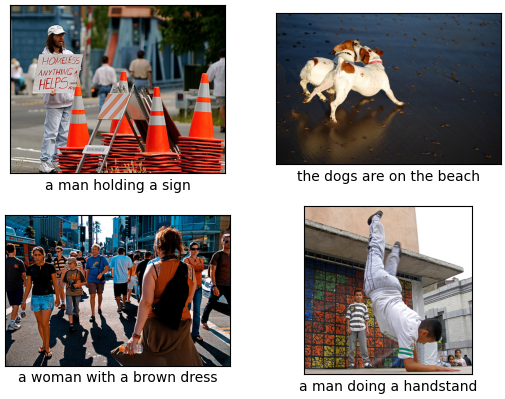
\includegraphics[width=.9\linewidth,trim={0 5cm 0 0},clip]{results/git_results}
  \caption{Przykładowe obrazy wraz z prostymi podpisami. Opracowanie własne.}
  \label{fig:sample-captions}
\end{figure}
\noindent Przedstawione powyżej opisy jasno wyrażają, co znajduje się na zdjęciach, ale brakuje w nich informacji np. o emocjach, otoczeniu itp. W głównej mierze opis sprowadza się do zidentyfikowania obiektów oraz czynności, jakie wykonują. Architektura ConCap pozwala na dodanie wraz ze zdjęciem zdania opisującego, jakiego tekstu byśmy oczekiwali, na przykład pozytywnego, czy też negatywnego. Przykłady różnego rodzaju opisów zostały przedstawione na rysunku \ref{fig:concap-captions}
\begin{figure}[H]
  \centering
  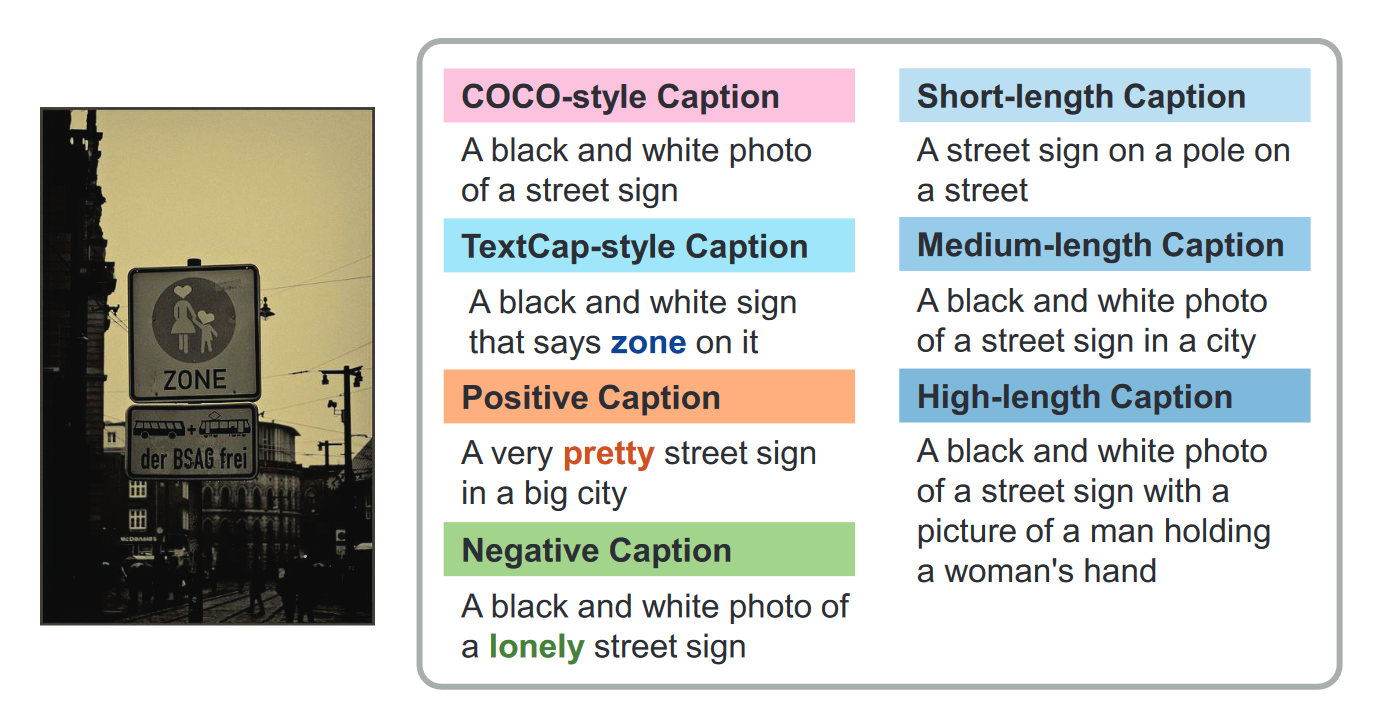
\includegraphics[width=.9\linewidth]{concap_captions}
  \caption{Różnego rodzaju opisy wygenerowane przez model ConCap. Źródło: \cite{concap}}
  \label{fig:concap-captions}
\end{figure}
\noindent Architektura ConCap składa się z między innymi transformera wizyjnego oraz sieci BERT \cite{bert}. Niestety autorzy nie wskazali, jaką wydajność osiąga ich rozwiązanie, jednakże można przypuszczać, iż ze względu na wykorzystanie kilku niezwykle rozbudowanych oraz obciążających obliczeniowo architektur, użycie tego rozwiązania wymaga sporych zasobów komputerowych. Sami autorzy w celach uczenia architektury wykorzystali 32 karty graficzne Nvidia V100, które są specjalistycznymi jednostkami obliczeniowymi. Skuteczność architektury waha się w zależności od rodzaju opisów, jakie były generowane, co jest dość zrozumiałe, ponieważ opisy pochodzące ze zbioru MS COCO są proste i podobieństwo wygenerowanych wartości w przypadku chęci wygenerowania na przykład pozytywnych opisów może znacznie bardziej się różnić niż w przypadku klasycznej generacji. Niemniej jednak architektura dla zbioru MS COCO generując proste opisy, osiągnęła wartość metryki BLEU-4 równą 0,41, co jest wynikiem porównywalnym do pozostałych architektur jak OFA czy GIT. W przypadku generowania długich opisów architektura osiągnęła najsłabszy wynik wynoszący 0,27, co i tak jest niezwykle dobrym rezultatem.

\subsection{Wydajność aktualnych rozwiązań}
Publikowanych jest coraz więcej artykułów dotyczących uczenia maszynowego, jednakże ciężko jest znaleźć publikacje podejmujące problem, jakim są wysokie wymagania sprzętowe potrzebne do stworzenia takiego rozwiązania, jak również jego wykorzystywania. Najczęściej w przypadku opisywania autorskiej architektury sieci neuronowej, autorzy podają ramy czasowe poświęcone na trenowanie architektury wraz z nazwą wykorzystywanej jednostki GPU. O wiele rzadziej pojawia się informacja o samym czasie potrzebnym do przetworzenia pojedynczej wartości wejściowej w kontekście późniejszego wykorzystywania proponowanego rozwiązania.
Przykładem publikacji, które poruszają problem wysokich wymagań sprzętowych rozwiązań dotyczących neuronowych sieci splotowych oraz rekurencyjnych są:
\begin{itemize}
  \item Analiza wydajności splotowych sieci neuronowych bazujących na GPU \cite{cnn-compare},
  \item Optymalizacja wydajności rekurencyjnych sieci neuronowych wykorzystujących GPU \cite{rnn-compare}.
\end{itemize}
Niestety ze względu na o wiele mniejszą popularność dziedziny generowania podpisów do obrazków, ciężko znaleźć badania dotyczące konkretnie tego problemu. W łatwy sposób można oszacować, w jakich proporcjach zmieniać będzie się sama wydajność wykorzystywanych architektur poprzez połączenie czasów jednego modułu wraz z czasami drugiego modułu otrzymanymi z istniejących badaniach. Mimo wszystko takich wyników nie można uznać za dokładne ze względu na konieczność wprowadzenia modyfikacji w konkretnych architekturach modułów, jak również zupełnie różne środowiska testowe wykorzystywane w konkretnych badaniach. Dodatkowym problemem jest brak informacji o skuteczności danej architektur w kontekście zastosowanych zasobów, co jest niezwykle istotnym aspektem, ponieważ w przypadku osiągnięcie niezwykle wydajnej architektury jednocześnie może ona osiągać o wiele słabszą dokładność generowanych wyników.
